\section{Methodology}


\subsection{Test Environment}
In our experiments, we were using the ODROID-X2 \cite{odroid-x2} developer
platform, which has an Exynos 4412 "Prime" System-on-Chip with four ARM
Cortex-A9 (r3p0) processor cores. We disable CPU core 1 through 3, leaving only
one core configured to run at a static frequency of $1.7$ GHz.

The Cortex-A9 is a 32-bit out-of-order dual-issue speculative RISC processor
with many features common for modern processor designs, making it attractive for
our experiments. After the dispatch stage, its pipeline is split into four
different lanes, each with its own functional units. Documentation on the
internal structure of the pipelines are not publicly available, but by running
experiments similar to the ones presented in \cite{paper} (explained below) and
looking at previous work\cite{armtech}\cite{7cpu}\cite{lotofdocs}, we are able
to get some details. The four pipelines are structured as follow: Main execution
pipeline with a general ALU, and a hardware-multiply, secondary execution
pipeline with only a general ALU, load-store-pipeline, containing only an
hardware adder to generate addresses, and a floating-point pipeline containing
an ordinary FPU and connections to the NEON unit.

The A9 processor has 58 distinct events that each can be mapped to one of six
generic event counters in the Performance Monitor Unit (i.e. only six generic
events can be tracked simultaneously). It also has a separate cycle counter. A
complete overview can be seen in table $A.18$ in the Cortex-A9 Technical
Reference Manual \cite{armtech}.


\todo[inline]{Move and rewrite this paragraph.}
It is a common philosophy that a RISC should consume one clock cycle pr.
instruction\cite{unknown}. For this particular processor made by Advanced RISC
Machines, it is not the case. The dual issue and its parallell general ALU
pipelines enables the processor to achive more than one instruction pr. clock
cycle, and at the same time, it supports multiply, divide and floating point,
each taking multiple clock cycles. It is even so that multiply, divide and
floating point takes different amount of cycles according to their surrounding
instructions.

\begin{figure}
% Graphic for TeX using PGF
% Title: /backup/hvatum/Skole/arm-project/report/figures/test_setup.xml
% Creator: Dia v0.97.2
% CreationDate: Wed Dec 11 22:34:20 2013
% For: hvatum
% \usepackage{tikz}
% The following commands are not supported in PSTricks at present
% We define them conditionally, so when they are implemented,
% this pgf file will use them.
\ifx\du\undefined
  \newlength{\du}
\fi
\setlength{\du}{15\unitlength}
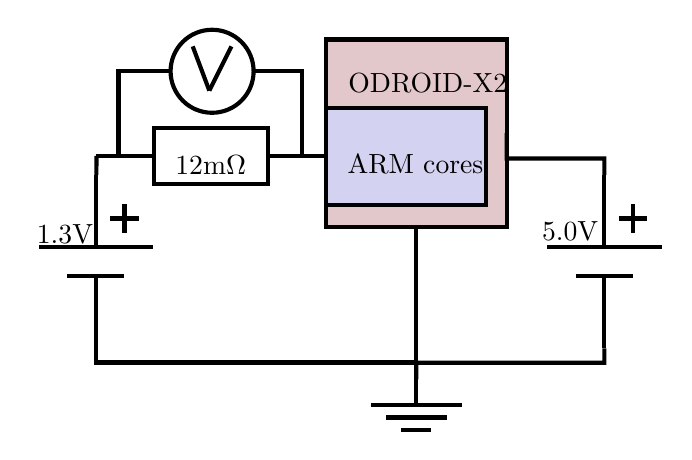
\begin{tikzpicture}
\pgftransformxscale{1.000000}
\pgftransformyscale{-1.000000}
\definecolor{dialinecolor}{rgb}{0.000000, 0.000000, 0.000000}
\pgfsetstrokecolor{dialinecolor}
\definecolor{dialinecolor}{rgb}{1.000000, 1.000000, 1.000000}
\pgfsetfillcolor{dialinecolor}
\pgfsetlinewidth{0.100000\du}
\pgfsetdash{}{0pt}
\pgfsetdash{}{0pt}
\pgfsetbuttcap
\pgfsetmiterjoin
\pgfsetlinewidth{0.100000\du}
\pgfsetbuttcap
\pgfsetmiterjoin
\pgfsetdash{}{0pt}
\definecolor{dialinecolor}{rgb}{0.000000, 0.000000, 0.000000}
\pgfsetstrokecolor{dialinecolor}
\draw (19.962100\du,12.768751\du)--(21.337939\du,12.768751\du);
\pgfsetbuttcap
\pgfsetmiterjoin
\pgfsetdash{}{0pt}
\definecolor{dialinecolor}{rgb}{1.000000, 1.000000, 1.000000}
\pgfsetfillcolor{dialinecolor}
\fill (21.337939\du,12.097000\du)--(21.337939\du,13.440503\du)--(24.089616\du,13.440503\du)--(24.089616\du,12.097000\du)--cycle;
\definecolor{dialinecolor}{rgb}{0.000000, 0.000000, 0.000000}
\pgfsetstrokecolor{dialinecolor}
\draw (21.337939\du,12.097000\du)--(21.337939\du,13.440503\du)--(24.089616\du,13.440503\du)--(24.089616\du,12.097000\du)--cycle;
\pgfsetbuttcap
\pgfsetmiterjoin
\pgfsetdash{}{0pt}
\definecolor{dialinecolor}{rgb}{0.000000, 0.000000, 0.000000}
\pgfsetstrokecolor{dialinecolor}
\draw (24.089616\du,12.768751\du)--(25.465455\du,12.768751\du);
% setfont left to latex
\definecolor{dialinecolor}{rgb}{0.000000, 0.000000, 0.000000}
\pgfsetstrokecolor{dialinecolor}
\node[anchor=west] at (18.254748\du,14.648958\du){1.3V};
% setfont left to latex
\definecolor{dialinecolor}{rgb}{0.000000, 0.000000, 0.000000}
\pgfsetstrokecolor{dialinecolor}
\node[anchor=west] at (18.254748\du,15.448958\du){};
\pgfsetlinewidth{0.100000\du}
\pgfsetdash{}{0pt}
\pgfsetdash{}{0pt}
\pgfsetbuttcap
\pgfsetmiterjoin
\pgfsetlinewidth{0.100000\du}
\pgfsetbuttcap
\pgfsetmiterjoin
\pgfsetdash{}{0pt}
\definecolor{dialinecolor}{rgb}{0.890196, 0.784314, 0.796078}
\pgfsetfillcolor{dialinecolor}
\fill (25.484300\du,9.968170\du)--(25.484300\du,14.476173\du)--(29.846883\du,14.476173\du)--(29.846883\du,9.968170\du)--cycle;
\definecolor{dialinecolor}{rgb}{0.000000, 0.000000, 0.000000}
\pgfsetstrokecolor{dialinecolor}
\draw (25.484300\du,9.968170\du)--(25.484300\du,14.476173\du)--(29.846883\du,14.476173\du)--(29.846883\du,9.968170\du)--cycle;
\pgfsetbuttcap
\pgfsetmiterjoin
\pgfsetdash{}{0pt}
\definecolor{dialinecolor}{rgb}{0.000000, 0.000000, 0.000000}
\pgfsetstrokecolor{dialinecolor}
\draw (25.484300\du,9.968170\du)--(25.484300\du,14.476173\du)--(29.846883\du,14.476173\du)--(29.846883\du,9.968170\du)--cycle;
% setfont left to latex
\definecolor{dialinecolor}{rgb}{0.000000, 0.000000, 0.000000}
\pgfsetstrokecolor{dialinecolor}
\node[anchor=west] at (25.759875\du,11.008700\du){ODROID-X2};
\pgfsetlinewidth{0.100000\du}
\pgfsetdash{}{0pt}
\pgfsetdash{}{0pt}
\pgfsetmiterjoin
\definecolor{dialinecolor}{rgb}{0.827451, 0.823529, 0.941176}
\pgfsetfillcolor{dialinecolor}
\fill (25.486700\du,11.611400\du)--(25.486700\du,13.961400\du)--(29.337189\du,13.961400\du)--(29.337189\du,11.611400\du)--cycle;
\definecolor{dialinecolor}{rgb}{0.000000, 0.000000, 0.000000}
\pgfsetstrokecolor{dialinecolor}
\draw (25.486700\du,11.611400\du)--(25.486700\du,13.961400\du)--(29.337189\du,13.961400\du)--(29.337189\du,11.611400\du)--cycle;
% setfont left to latex
\definecolor{dialinecolor}{rgb}{0.000000, 0.000000, 0.000000}
\pgfsetstrokecolor{dialinecolor}
\node[anchor=west] at (25.737200\du,12.964800\du){ARM cores};
% setfont left to latex
\definecolor{dialinecolor}{rgb}{0.000000, 0.000000, 0.000000}
\pgfsetstrokecolor{dialinecolor}
\node[anchor=west] at (30.423200\du,14.580700\du){5.0V};
\pgfsetlinewidth{0.100000\du}
\pgfsetdash{}{0pt}
\pgfsetdash{}{0pt}
\pgfsetbuttcap
\pgfsetmiterjoin
\pgfsetlinewidth{0.100000\du}
\pgfsetbuttcap
\pgfsetmiterjoin
\pgfsetdash{}{0pt}
\definecolor{dialinecolor}{rgb}{0.000000, 0.000000, 0.000000}
\pgfsetstrokecolor{dialinecolor}
\draw (27.667052\du,18.153700\du)--(27.667052\du,18.766668\du);
\pgfsetbuttcap
\pgfsetmiterjoin
\pgfsetdash{}{0pt}
\definecolor{dialinecolor}{rgb}{0.000000, 0.000000, 0.000000}
\pgfsetstrokecolor{dialinecolor}
\draw (26.568500\du,18.766668\du)--(28.765605\du,18.766668\du);
\pgfsetbuttcap
\pgfsetmiterjoin
\pgfsetdash{}{0pt}
\definecolor{dialinecolor}{rgb}{0.000000, 0.000000, 0.000000}
\pgfsetstrokecolor{dialinecolor}
\draw (26.936515\du,19.073151\du)--(28.397590\du,19.073151\du);
\pgfsetbuttcap
\pgfsetmiterjoin
\pgfsetdash{}{0pt}
\definecolor{dialinecolor}{rgb}{0.000000, 0.000000, 0.000000}
\pgfsetstrokecolor{dialinecolor}
\draw (27.304530\du,19.379635\du)--(28.029575\du,19.379635\du);
% setfont left to latex
\definecolor{dialinecolor}{rgb}{0.000000, 0.000000, 0.000000}
\pgfsetstrokecolor{dialinecolor}
\node at (22.713800\du,12.990050\du){12m$\Omega$};
\pgfsetlinewidth{0.100000\du}
\pgfsetdash{}{0pt}
\pgfsetdash{}{0pt}
\pgfsetbuttcap
\pgfsetmiterjoin
\pgfsetlinewidth{0.100000\du}
\pgfsetbuttcap
\pgfsetmiterjoin
\pgfsetdash{}{0pt}
\definecolor{dialinecolor}{rgb}{1.000000, 1.000000, 1.000000}
\pgfsetfillcolor{dialinecolor}
\pgfpathellipse{\pgfpoint{22.747033\du}{10.732410\du}}{\pgfpoint{1.000000\du}{0\du}}{\pgfpoint{0\du}{1.000000\du}}
\pgfusepath{fill}
\definecolor{dialinecolor}{rgb}{0.000000, 0.000000, 0.000000}
\pgfsetstrokecolor{dialinecolor}
\pgfpathellipse{\pgfpoint{22.747033\du}{10.732410\du}}{\pgfpoint{1.000000\du}{0\du}}{\pgfpoint{0\du}{1.000000\du}}
\pgfusepath{stroke}
\pgfsetbuttcap
\pgfsetmiterjoin
\pgfsetdash{}{0pt}
\definecolor{dialinecolor}{rgb}{0.000000, 0.000000, 0.000000}
\pgfsetstrokecolor{dialinecolor}
\draw (22.680367\du,11.199077\du)--(23.213700\du,10.132410\du);
\pgfsetbuttcap
\pgfsetmiterjoin
\pgfsetdash{}{0pt}
\definecolor{dialinecolor}{rgb}{0.000000, 0.000000, 0.000000}
\pgfsetstrokecolor{dialinecolor}
\draw (22.680367\du,11.199077\du)--(22.280367\du,10.132410\du);
\pgfsetbuttcap
\pgfsetmiterjoin
\pgfsetdash{}{0pt}
\definecolor{dialinecolor}{rgb}{0.000000, 0.000000, 0.000000}
\pgfsetstrokecolor{dialinecolor}
\draw (20.613700\du,10.732410\du)--(21.747033\du,10.732410\du);
\pgfsetbuttcap
\pgfsetmiterjoin
\pgfsetdash{}{0pt}
\definecolor{dialinecolor}{rgb}{0.000000, 0.000000, 0.000000}
\pgfsetstrokecolor{dialinecolor}
\draw (23.747033\du,10.732410\du)--(24.880367\du,10.732410\du);
\pgfsetlinewidth{0.100000\du}
\pgfsetdash{}{0pt}
\pgfsetdash{}{0pt}
\pgfsetbuttcap
\pgfsetmiterjoin
\pgfsetlinewidth{0.100000\du}
\pgfsetbuttcap
\pgfsetmiterjoin
\pgfsetdash{}{0pt}
\definecolor{dialinecolor}{rgb}{0.000000, 0.000000, 0.000000}
\pgfsetstrokecolor{dialinecolor}
\draw (32.197597\du,13.236300\du)--(32.197597\du,14.973868\du);
\pgfsetbuttcap
\pgfsetmiterjoin
\pgfsetdash{}{0pt}
\definecolor{dialinecolor}{rgb}{0.000000, 0.000000, 0.000000}
\pgfsetstrokecolor{dialinecolor}
\draw (30.819800\du,14.973868\du)--(33.575394\du,14.973868\du);
\pgfsetbuttcap
\pgfsetmiterjoin
\pgfsetdash{}{0pt}
\definecolor{dialinecolor}{rgb}{0.000000, 0.000000, 0.000000}
\pgfsetstrokecolor{dialinecolor}
\draw (31.508699\du,15.668895\du)--(32.886496\du,15.668895\du);
\pgfsetbuttcap
\pgfsetmiterjoin
\pgfsetdash{}{0pt}
\definecolor{dialinecolor}{rgb}{0.000000, 0.000000, 0.000000}
\pgfsetstrokecolor{dialinecolor}
\draw (32.886496\du,13.931327\du)--(32.886496\du,14.626354\du);
\pgfsetbuttcap
\pgfsetmiterjoin
\pgfsetdash{}{0pt}
\definecolor{dialinecolor}{rgb}{0.000000, 0.000000, 0.000000}
\pgfsetstrokecolor{dialinecolor}
\draw (32.542046\du,14.278841\du)--(33.230945\du,14.278841\du);
\pgfsetbuttcap
\pgfsetmiterjoin
\pgfsetdash{}{0pt}
\definecolor{dialinecolor}{rgb}{0.000000, 0.000000, 0.000000}
\pgfsetstrokecolor{dialinecolor}
\draw (32.197597\du,15.668895\du)--(32.197597\du,17.406462\du);
\pgfsetlinewidth{0.100000\du}
\pgfsetdash{}{0pt}
\pgfsetdash{}{0pt}
\pgfsetbuttcap
\pgfsetmiterjoin
\pgfsetlinewidth{0.100000\du}
\pgfsetbuttcap
\pgfsetmiterjoin
\pgfsetdash{}{0pt}
\definecolor{dialinecolor}{rgb}{0.000000, 0.000000, 0.000000}
\pgfsetstrokecolor{dialinecolor}
\draw (19.947397\du,13.236300\du)--(19.947397\du,14.973868\du);
\pgfsetbuttcap
\pgfsetmiterjoin
\pgfsetdash{}{0pt}
\definecolor{dialinecolor}{rgb}{0.000000, 0.000000, 0.000000}
\pgfsetstrokecolor{dialinecolor}
\draw (18.569600\du,14.973868\du)--(21.325194\du,14.973868\du);
\pgfsetbuttcap
\pgfsetmiterjoin
\pgfsetdash{}{0pt}
\definecolor{dialinecolor}{rgb}{0.000000, 0.000000, 0.000000}
\pgfsetstrokecolor{dialinecolor}
\draw (19.258499\du,15.668895\du)--(20.636296\du,15.668895\du);
\pgfsetbuttcap
\pgfsetmiterjoin
\pgfsetdash{}{0pt}
\definecolor{dialinecolor}{rgb}{0.000000, 0.000000, 0.000000}
\pgfsetstrokecolor{dialinecolor}
\draw (20.636296\du,13.931327\du)--(20.636296\du,14.626354\du);
\pgfsetbuttcap
\pgfsetmiterjoin
\pgfsetdash{}{0pt}
\definecolor{dialinecolor}{rgb}{0.000000, 0.000000, 0.000000}
\pgfsetstrokecolor{dialinecolor}
\draw (20.291846\du,14.278841\du)--(20.980745\du,14.278841\du);
\pgfsetbuttcap
\pgfsetmiterjoin
\pgfsetdash{}{0pt}
\definecolor{dialinecolor}{rgb}{0.000000, 0.000000, 0.000000}
\pgfsetstrokecolor{dialinecolor}
\draw (19.947397\du,15.668895\du)--(19.947397\du,17.406462\du);
\pgfsetlinewidth{0.100000\du}
\pgfsetdash{}{0pt}
\pgfsetdash{}{0pt}
\pgfsetbuttcap
{
\definecolor{dialinecolor}{rgb}{0.000000, 0.000000, 0.000000}
\pgfsetfillcolor{dialinecolor}
% was here!!!
\definecolor{dialinecolor}{rgb}{0.000000, 0.000000, 0.000000}
\pgfsetstrokecolor{dialinecolor}
\draw (19.962100\du,12.768800\du)--(19.959407\du,13.236300\du);
}
\pgfsetlinewidth{0.100000\du}
\pgfsetdash{}{0pt}
\pgfsetdash{}{0pt}
\pgfsetmiterjoin
\pgfsetbuttcap
{
\definecolor{dialinecolor}{rgb}{0.000000, 0.000000, 0.000000}
\pgfsetfillcolor{dialinecolor}
% was here!!!
{\pgfsetcornersarced{\pgfpoint{0.000000\du}{0.000000\du}}\definecolor{dialinecolor}{rgb}{0.000000, 0.000000, 0.000000}
\pgfsetstrokecolor{dialinecolor}
\draw (29.846900\du,12.222200\du)--(29.846900\du,12.833100\du)--(32.197516\du,12.833100\du)--(32.197529\du,13.236170\du);
}}
\pgfsetlinewidth{0.100000\du}
\pgfsetdash{}{0pt}
\pgfsetdash{}{0pt}
\pgfsetmiterjoin
\pgfsetbuttcap
{
\definecolor{dialinecolor}{rgb}{0.000000, 0.000000, 0.000000}
\pgfsetfillcolor{dialinecolor}
% was here!!!
{\pgfsetcornersarced{\pgfpoint{0.000000\du}{0.000000\du}}\definecolor{dialinecolor}{rgb}{0.000000, 0.000000, 0.000000}
\pgfsetstrokecolor{dialinecolor}
\draw (19.947400\du,17.406500\du)--(19.947400\du,17.747500\du)--(27.667100\du,17.747500\du)--(27.667100\du,18.153700\du);
}}
\pgfsetlinewidth{0.100000\du}
\pgfsetdash{}{0pt}
\pgfsetdash{}{0pt}
\pgfsetmiterjoin
\pgfsetbuttcap
{
\definecolor{dialinecolor}{rgb}{0.000000, 0.000000, 0.000000}
\pgfsetfillcolor{dialinecolor}
% was here!!!
{\pgfsetcornersarced{\pgfpoint{0.000000\du}{0.000000\du}}\definecolor{dialinecolor}{rgb}{0.000000, 0.000000, 0.000000}
\pgfsetstrokecolor{dialinecolor}
\draw (27.667100\du,18.153700\du)--(27.667100\du,17.754200\du)--(32.197514\du,17.754200\du)--(32.197526\du,17.404957\du);
}}
\pgfsetlinewidth{0.100000\du}
\pgfsetdash{}{0pt}
\pgfsetdash{}{0pt}
\pgfsetmiterjoin
\pgfsetbuttcap
{
\definecolor{dialinecolor}{rgb}{0.000000, 0.000000, 0.000000}
\pgfsetfillcolor{dialinecolor}
% was here!!!
{\pgfsetcornersarced{\pgfpoint{0.000000\du}{0.000000\du}}\definecolor{dialinecolor}{rgb}{0.000000, 0.000000, 0.000000}
\pgfsetstrokecolor{dialinecolor}
\draw (21.462300\du,10.732400\du)--(20.492500\du,10.732400\du)--(20.492500\du,12.768800\du)--(20.810700\du,12.768800\du);
}}
\pgfsetlinewidth{0.100000\du}
\pgfsetdash{}{0pt}
\pgfsetdash{}{0pt}
\pgfsetmiterjoin
\pgfsetbuttcap
{
\definecolor{dialinecolor}{rgb}{0.000000, 0.000000, 0.000000}
\pgfsetfillcolor{dialinecolor}
% was here!!!
{\pgfsetcornersarced{\pgfpoint{0.000000\du}{0.000000\du}}\definecolor{dialinecolor}{rgb}{0.000000, 0.000000, 0.000000}
\pgfsetstrokecolor{dialinecolor}
\draw (24.880400\du,10.732400\du)--(24.911900\du,10.732400\du)--(24.911900\du,12.768800\du)--(25.465500\du,12.768800\du);
}}
\pgfsetlinewidth{0.100000\du}
\pgfsetdash{}{0pt}
\pgfsetdash{}{0pt}
\pgfsetmiterjoin
\pgfsetbuttcap
{
\definecolor{dialinecolor}{rgb}{0.000000, 0.000000, 0.000000}
\pgfsetfillcolor{dialinecolor}
% was here!!!
{\pgfsetcornersarced{\pgfpoint{0.000000\du}{0.000000\du}}\definecolor{dialinecolor}{rgb}{0.000000, 0.000000, 0.000000}
\pgfsetstrokecolor{dialinecolor}
\draw (27.665592\du,14.476173\du)--(27.665592\du,16.314936\du)--(27.667052\du,16.314936\du)--(27.667052\du,18.153700\du);
}}
\end{tikzpicture}

\caption{Test Setup}
\label{fig:setup}
\end{figure}

\subsection{Architectural Experiments}
\label{arch_experiments}
Running the processor at it's highest possible throughput requires knowledge of
internal components in the pipeline, e.g. to find out the number of $add$s it is
capable of doing per cycle. As we are using a proprietary platform as our target
architecture, only some of these details are known. Thus, we define test
programs to stress particular pipeline components and gather statistics using
performance counters. By comparing execution unit counters and the total cycle
count, we obtain detailed (although approximate, due to the speculativity in the
core) information of a test program's execution.
\todo[inline]{Elaborate in detail, see notes/alu-count.txt.}

Using the same approach as above, we are able to identify a feature on the A9
processor that is very vaguely documented; fast-loop\texttrademark mode. As the
name suggests, this feature enables rapid execution of small loops by bypassing
the L1 cache.  However, which loops that falls into this category is not
documented, but by using performance counters we are able to determine this with
confidence.
\todo[inline]{Add appendix explaining fast-loop microbenchmark.}


\subsection{Benchmarks}
As a first approximation, the benchmark programs consists of an infinite series
of identic instructions. The A9 core runs at a fixed frequency and we are
providing a fixed core voltage, so energy usage of simple, one-cycle instruction
could be retrieved by running for a fixed time period and applying the following
formula.

\todo{fix formula}
\begin{equation}
    P_{instruction} = A_{instruction} \cdot V_{core}
\end{equation}
\begin{equation}
    E_{instruction} = P_{instruction} \cdot CPI_{instruction}
\end{equation}
The Agilent multimeter is set up to sample at full precision at its maximum rate
of 1000 Hz. This yields one sample every $\frac{ f_{core} }{ 1000 } = 1.7$
million instructions; it is obvious from this that we are unable to observe
inter-cycle variations in energy consumption.
\todo[inline]{But maybe the multimeter is doing a running average internally?}

This simple setup does not take the memory system into account; we are
undoubtedly not able to feed the processor instructions at no cost in terms of
access speed and -- more importantly -- memory system energy usage. Thus, we
improve this model by investigating features that avoids the memory system as
much as possible.

Furthermore, executing code within fast-loop allows us to limit the number of
cache mispredicts to 2, independently of the iteration count.
\todo[inline]{Explain how and why these to misses occur}

\begin{figure}
\begin{lstlisting}{language=[ARM]Assembler}
label: instruction
       . . .
       instruction
       subs
       jne label
\end{lstlisting}
\caption{Instruction loop}
\label{list:inst_loop}
\end{figure}

\subsection{Power Measurements}
To measure energy consumption, we use an Agilent 34410A multimeter and measures
voltage drop over a negligible $12$ $m\Omega$ resistor. We decouple power
consumption on the ARM cores and the development board by modifying the
ODROID-X2 and providing a separate power supply for the A9 cores. They get
powered by an external power supply giving $1.3V$ DC, while the rest of the
board is powered from a another power supply at $5.0V$, as depicted in figure
\todo{figure ref}.

\subsection{Pit Falls}
% temperature, noise (inducted power, etc.), interrupts, memory latency (fast-loop)
Since we are comparing the energy efficency of different instruction in an asynchronous
way, we have to consider factors that affects power usage, as well as acknowledege that
they may differ between runs.

One obviuos such factor is temperature, both ambient and
the chip temperature. The first may change without our notice, and the second one is
determined by the ambient, the cooling device and what load tasks that was just run on
the SoC. On this specific SoC, Samsung Exynos 4412, we have detected that the difference
from the CPU Thermal Zone 0 being 9$^\circ$ Celcius and 63$^\circ$ Celcius is on average
between 2-4\%. We also detected that some instructions might have as much as 7\% higher
energy consumption when running at the hotter level\footnote{This was detected with at
the {\ttfamily mul}-instruction}. We have also checked that running a single core at
maximum performace over time does not increase the temperature by more than from
idle at 47$^\circ$ Celcius to 54$^\circ$ Celcius at load. Assuming that it is generally
true that a single core cannot heat the entire SoC with any significant amount, and that
the increase in power consumption is at max 10\% over 50$^\circ$ Celcius, we get
\begin{equation}
    P_{inc} = P_{orig} \cdot T_{inc} \cdot \frac{0.10}{50} = P_{orig} \cdot T_{inc} \cdot 0.002
\end{equation}
Believing that this trend is at least close to linear, output will increase by 0.2\% pr.
degree Celcius increased. Also, we start our measurements at leat half a second after the benchmarks
have been started, thus there is plenty of time for the CPU to gain work temperature. In our
tests, the time used to get to work temperature was humanly instant.

Another factor that is not that obvious, but at least equally important, is power inducted
in the measurement circuit. Since wires are often winded up on the test bench, and lab equipment
might contain large metal cores with a great amount of power running through them, unexpected
power might be introduced.

We are running Linux on the chip under test, this gives us a much simpler way of programming
the processor to run our tests. The fact that we run an entire operating system benith our
benchmark programs implies that there is much going on that we have no direct controll over.
In order to mitigate the artifacts originating from the operating system, we
disable all the maskable interrupts.

As explained in section \ref{arch_experiments}, we utilize the fast-loop mode of the processor to mitigate
memory access latencies. We disable the L1 cache to easier detect when we are outside the fast-loop mode,
and thus we are certain that there is no memory access going on.
